The first step of the evaluation was to perform a 10-fold cross-validation in
order to find the decision tree's performance. Using the cross-validation we
found out that the average error of the 10 estimates is 10\%. 

Since we have already calculated the predicted subsets from the table examples, we can easily calculate the confusion matrix. To be more specific, we concatenate the 10 predicted subsets and we use them as input, along with the actual target labels, to the general purpose function which is responsible for the calculation of the confusion matrix.  As a result we retrieved the matrix below which is the confusion matrix for the 10-fold validation.
See figure~\ref{fig:confusionMatrix}.
\include*{confusion_matrix}

From this matrix we can observe that the correct classifications for each
class-emotion are on the matrix's diagonal. So we can conclude that for the
Surprise and for the Happiness there isn't any confusion. On the other hand, for the Anger, Disgust, Fear and Sadness there are some misclassified examples. 

For the calculation of the precision and the recall rates per class, we used two formulas which can use the information we already have in the confusion matrix and calculate those two rates.

See figure~\ref{fig:averageRecall}
\include*{average_recall_precision}

So for example we have the confusion matrix below:

\begin{figure}[h]
    \centering
    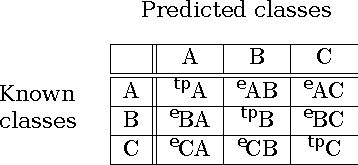
\includegraphics[width=0.3\textwidth]{confusionMatrixCalc.pdf}
    \caption{TITLE HERE}
    \label{fig:confisionMatixCalc}
\end{figure}

We can easily derive the recall and the precision by using those formulas:

Precision\textsubscript{A} = tp\textsubscript{A}/(tp\textsubscript{A}+e\textsubscript{BA}+e\textsubscript{CA})

Recall\textsubscript{A} = tp\textsubscript{A}/(tp\textsubscript{A}+e\textsubscript{AB}+e\textsubscript{AC})

(The precision and recall rates, along with the F1-measure proof our previous conclusions for classes-emotions.)
